\documentclass[ngerman]{article}

\usepackage{xcolor}
\usepackage[T1]{fontenc}
\usepackage{pgffor}
\usepackage{todonotes}
\usepackage{minted}
\usepackage{graphicx}
\usepackage{minted}
\usemintedstyle{vs}
\usepackage{fancyhdr}
\usepackage{hyperref}
\usepackage{tcolorbox}
\usepackage{etoolbox}
\usepackage[margin=1.2in]{geometry}
\usepackage[ngerman]{babel} 
\usepackage{inconsolata}
\usepackage{bookmark}
\usepackage{wrapfig} 
\usepackage{lipsum}
\usepackage[autolang=other, backend=biber]{biblatex}
\addbibresource{refs.bib}

\hypersetup{
  colorlinks=true,
  linkcolor=blue,
  filecolor=magenta,
  citecolor=blue,
  urlcolor=blue,
}

\renewcommand*\familydefault{\ttdefault} %% Only if the base font of the document is to be typewriter style

\newcommand{\topic}[1]{\tcbox[on line,arc=4pt,colframe=white,boxrule=0pt,boxsep=0pt,left=4pt,right=4pt,top=3pt,bottom=2pt,colback=gray!30]{#1}}

\newcommand{\br}{\linebreak\linebreak}

\newcommand{\link}[2][]{%
    \ifblank{#1}{%
        \hyperref[sec:#2]{#2}%
    }{%
        \hyperref[sec:#1]{#2}%
    }%
}

\newenvironment{code}
  {%
    \begin{tcolorbox}[
        colback=white,
        colframe=black,
        boxrule=0.5pt,
        arc=4pt,
        left=2mm,
        right=2mm,
        top=2mm,
        bottom=2mm,
      ]
      }{% 
    \end{tcolorbox}
    }


\newcommand{\cmt}[1]{\textcolor{gray!60}{\textit{/* #1 */}}}

\newcommand{\qt}[1]{„#1“}

% Define a custom command for colored boxes around words
\newcommand{\topics}[1]{%
  \linebreak
  \linebreak
  \foreach \word in {#1} {%
    \topic{\word}%
  }%
  \linebreak
}


\title{Bachelorarbeit}
\author{Max Richter}

\begin{document}

\pagestyle{fancy}
\fancyhead{} % clear all header fields
\fancyhead[RO,LE]{\textbf{WebAssembly-basierte visuelle Programmiersprache}}
\fancyfoot{} % clear all footer fields
\fancyfoot[LE,RO]{\thepage}
\fancyfoot[LO,CE]{\href{https://github.com/jim-fx/bachelor}{github.com/jim-fx/bachelor}}
\fancyfoot[CO,RE]{Max Richter}

\raggedright

\maketitle
\pagebreak

\tableofcontents

\pagebreak

\section{Einleitung}

\subsection{Hintergrund}
In unserer heutigen digitalisierten Welt spielen Human-Computer Interfaces (HCI's) eine entscheidende Rolle.
Hierbei gibt es eine weite Spanne von Komplexität, von einfach zu bedienenden grafischen Benutzeroberflächen bis zu komplexen Programmiersprachen. 
\br
Da Menschen Konzepte und Relationen größtenteils visuell und räumlich verarbeiten \cite{smith1975pygmalion}, bieten visuelle Programmiersprachen (VPL's) einen guten Mittelweg für programmierunerfahrene Nutzer/innen. 
Sie vereinen die Benutzerfreundlichkeit grafischer Interfaces mit der Komplexität und Flexibilität textbasierter Programmiersprachen.
\br
Es gibt bereits eine Vielzahl von VPL's, die in unterschiedlichen Bereichen Anwendung finden. 
Diese reichen von einfachen Tools wie \textit{Scratch} für Kinder bis zu komplexen Systemen wie \textit{Blender} für 3D-Modellierung und Animation.
\br
In dieser Bachelorarbeit wird eine VPL entwickelt bei der die einzelnen Bausteine als WebAssembly-Module implementiert sind. 
Dies ermöglicht es neue Bausteine von anderen Entwickler/innen einfach hinzuzufügen und so die Funktionalität der VPL zu erweitern.
Hierbei garantiert WebAssembly eine hohe Performance und Sicherheit, da der Code in einer virtuellen Maschine ausgeführt wird.

\subsection{Problemstellung}

Die Entscheidung diese VPL als Webanwendung zu entwickeln wurde aus mehreren Gründen getroffen. 
Einerseits verfüge ich bereits über einige Erfahrung in der Entwicklung von Webanwendungen. 
Andererseits bietet das Web Nutzer/innen einen niedrigschwelligen Zugang zur Anwendung, da sie keine zusätzliche Software installieren müssen.
\br
Trotz dieser Vorteile bringt die Entwicklung von Webanwendungen auch spezifische Herausforderungen mit sich.
So ist die Sprache in der dynamische Webanwendungen entwickelt werden, Javascript, \qt{garbage-collected} und nicht stark typisiert. 
Dies macht es theoretisch schwieriger performante und robuste Anwendungen zu entwickeln. 
Um die Entwicklung etwas leichter zu gestalten habe ich mich entschieden die VPL in \link[TypeScript]{TypeScript} zu entwickeln, da diese Sprache stark typisiert ist und zu JavaScript kompiliert wird.
\br
Weitere Herausforderungen entstehen durch die Nutzung von WebAssembly. 
WebAssembly führt Code in einer virtuellen Maschine aus, die nicht direkt Zugang auf den Speicher oder Variablen der Host-Umgebung (den Browser) hat.
Innerhalb dieser virtuellen Maschine wird der Code nahe der nativen Geschwindigkeit ausgeführt, was zu einer hohen Performance führt. 
Die Herausforderung besteht darin das die Kommunikation zwischen der Host-Umgebung und dieser virtuellen Maschine relativ langsam ist und so zu einem Engpass führen kann.
\br
Außerdem erlaubt WebAssembly nur sehr wenige numerische Datentypen; 32 und 64 Bit Integer sowie 32 und 64 Bit Floats nach dem IEEE 754 Standard. 
Größere und komplexe Datentypen müssen serialisiert werden, um sie an WebAssembly zu übergeben. 
Um komplexere Werte wieder an die Host-Umgebung zu übergeben, muss diese direkt auf den Speicher der virtuellen Maschine zugreifen.
Zum Glück gibt es Bibliotheken wie \link[WASM-Bindgen]{WASM-Bindgen} die diese Kommunikation abstrahieren und vereinfachen.
\br
Da WebAssembly ein binäres Format ist, wird es selten direkt geschrieben und meistens als Kompilierungsziel für komplexere Programmiersprachen benutzt.
Ich entschied mich für die Programmiersprache \link[Rust]{Rust}, da sie eine starke Typisierung, Performance und Speicher-Sicherheit bietet \cite{bugden2022rust}.
Außerdem bietet \link[Rust]{Rust} eine gute Integration mit WebAssembly und ermöglicht es, Rust-Code direkt in WebAssembly zu kompilieren. 
Die \href{https://rustwasm.github.io/}{Rust and WebAssembly domain working group} bietet viele Tools und Bibliotheken an, die die Entwicklung von WebAssembly-Anwendungen in \link[Rust]{Rust} erleichtern.

\subsection{Zielsetzung} 
\label{sec:Zielsetzung}

Das Ziel dieser Bachelorarbeit ist es eine visuelle Programmiersprache zu entwickeln, die \textbf{performant}, \textbf{erweiterbar} und möglichst \textbf{einfach zu bedienen} ist.
Um diese drei Anforderungen laufend zu überprüfen wird die VPL im Kontext einer Web-App entwickelt die den Nutzer/innen erlaubt prozedurale 3D-Modelle von Pflanzen zu erstellen.
Dieser Anwendungsfall wurde gewählt da die hohen Datenmengen von 3D-Modellen eine gute Möglichkeit bieten die Performance der VPL zu testen.
\br
Ein weiteres Ziel dieser Arbeit ist es, die Eignung von WebAssembly als Grundlage für eine solche VPL zu untersuchen. 
Dadurch das WebAssembly plattformunabhängig ist und es sich eignet, um performante Anwendungen zu entwickeln, könnte es sich als Grundlage für eine VPL anbieten.

\subsection{Forschungsfragen}

Inwieweit eignet sich WebAssembly als Grundlage für eine node-basierte visuelle Programmiersprache?  
\br
Welche Auswirkungen haben die spezifischen Vor- und Nachteile von WebAssembly auf die Realisierbarkeit, Funktionalität, Nutzerfreundlichkeit, Performance, Flexibilität und Robustheit einer solchen Programmiersprache?

\section{Theoretischer Rahmen}

\subsection{Definition von visuellen Programmiersprachen}
Eine visuelle Programmiersprache stellt die Komponenten und Verbindungen eines Programms in mehr als einer Dimension dar. Oft ist diese Dimension eine zweidimensionale Fläche auf der die einzelnen Funktionen oder Komponenten eines Systems visuell dargestellt werden. \cite{Myers}
Auch wenn textuelle Sprache auf einer zweidimensionalen Oberfläche dargestellt wird, so ist sie meist aus Sicht des Interpreters oder Compilers ein eindimensionaler Stream aus Tokens.

\subsection{Klassifikation von visuellen Programmiersprachen}

Nach Burnett\&Mayer können VPL's in 5 verschiedenen Klassen eingeteilt werden \cite{BURNETT1994287}. Diese einzelnen Klassen schließen sich nicht gegenseitig aus und können auch in Kombination verwendet werden.

\subsubsection{\qt{Purely visual languages}}
\qt{Purely visual languages} haben keine textuelle Repräsentation und sind ausschließlich visuell. Ein Beispiel hierfür ist Scratch, das es Nutzern ermöglicht, durch das Zusammensetzen von Blöcken Programme zu erstellen, ohne eine einzige Zeile Code zu schreiben. \cite{mitScratchAbout}


\subsubsection{\qt{Hybrid text and visual Systems}}
\qt{Hybrid text and visual systems} haben eine textuelle Repräsentation, die parallel zur visuellen Repräsentation existiert. 
Ein Beispiel hierfür ist Microsoft's Visual Programming Language, das Teil von Microsoft Robotics Developer Studio ist und eine hybride Umgebung bietet, in der Nutzer sowohl Code schreiben als auch visuelle Elemente nutzen können. \cite{microsoftIntroduction}

\subsubsection{\qt{Programming-by-example Systems}}
Programming-by-example systems erlauben es dem Nutzer, ein Programm zu schreiben, indem er die gewünschte Funktionalität in einem Beispiel demonstriert. Etoys, basierend auf Squeak, ist ein Beispiel für ein solches System, bei dem Benutzer durch das Demonstrieren von Aktionen Objekte programmieren können. \cite{squeakSqueakSmalltalk}

\subsubsection{\qt{Constraint-oriented Systems}}
\qt{Constraint-oriented Systems} erlauben es dem Nutzer, Constraints zwischen den Komponenten des Programms zu definieren. SketchPad wäre ein Beispiel für ein solches System, bei dem Benutzer geometrische Formen zeichnen und Constraints zwischen ihnen definieren können. \cite{sutherlandSketchpad}


\subsubsection{\qt{Form-based systems}}
In \qt{Form-based systems} schreiben die Nutzer Programme, indem sie Formulare ausfüllen. 
Ein klassisches Beispiel für ein formular-basiertes System ist Oracle Forms, 
das eine GUI für Datenbankabfragen und -transaktionen bietet, indem es Benutzern ermöglicht, Formulare auszufüllen, die dann in SQL-Code umgewandelt werden. \cite{wikipediaOracleForms}

\subsection{Historische Vorbilder}

\subsubsection{SketchPad (1963)}
\label{sec:SketchPad}
\begingroup
\setlength\intextsep{4pt}
\begin{minipage}{\linewidth}
\begin{wrapfigure}{R}{0.5\textwidth}
  \centering
  \includegraphics[width=0.4\textwidth]{./graphics/sketchpad-sutherland.jpg} % Change example-image-a with your image filename
  \caption{SketchPad \cite{sutherlandSketchpad}}
\end{wrapfigure}
SketchPad ist ein von Ivan Sutherland entwickeltes Programm das 1963 am MIT veröffentlicht wurde. 
Es benutzte einen Lightpen als Eingabegerät und war das erste Programm, das die Interaktion mit einem Computer über eine grafische Benutzeroberfläche ermöglichte. 
Es erlaubte den Nutzer/innen, geometrische Formen auf einem Bildschirm zu zeichnen und diese zu manipulieren.
  Dabei existierten diese Formen auf einem virtuellen \qt{Papier}, dass der Nutzer bewegen und zoomen konnte. Dieses Konzept von bewegen und Zoomen virtueller Oberflächen war revolutionär für die damalige Zeit.
  Dies wird deutlich durch den Fakt das der Präsentator während der Präsentation von SketchPad \cite{sketchpadDemo} (10:30) keine Worte fand, um diesen Vorgang zu beschreiben.
Ein weiteres Feature war die Möglichkeit, Constraints zwischen den Formen zu definieren, ähnlich wie in modernen CAD-Programmen. 
Wenn man sich die Videodemo von SketchPad anschaut fallen viele Paradigmen auf, die wir heute als gegeben ansehen.
Auch wenn SketchPad nicht direkt in die Definition einer VPL passt, war es ein Meilenstein der Entwicklung von grafischen HCI's. Was durch die Verleihung des Turing Awards an Ivan Sutherland 1988 bestätigt wurde.
\end{minipage}
\endgroup

\subsubsection{Pygmalion (1970)}
\begingroup
\setlength\intextsep{2pt}
\begin{minipage}{\linewidth}
\begin{wrapfigure}{L}{0.4\textwidth}
  \centering
  \includegraphics[width=0.4\textwidth]{./graphics/pygmalion.jpg}
  \caption{Fakultät in Pygmalion \cite{smith1975pygmalion}}
  \label{fig:pygmalion_demo}
\end{wrapfigure}

Pygmalion ist eine visuelle Programmiersprache die um 1970 von David Canfield Smith im Rahmen seiner Doktorarbeit entwickelt wurde. Inspiriert wurde sie von der mythischen Figur des Bildhauers Pygmalion der seine Skulpturen zum Leben erwecken konnte.
Die Sprache erlangte nie eine große Verbreitung, war aber ein wichtiger Meilenstein in der Entwicklung von visuellen Programmiersprachen und HCI's.
Pygmalion wurde in Smalltalk implementiert und war eine der ersten visuellen Programmiersprachen. Über eine grafische Oberfläche konnten die Nutzer/innen Blöcke, Icons und Verbindungen erstellen und manipulieren im damit Programme zu definieren.
  Icons waren damals eine Neuerung und wurden von den Entwicklern als \qt{eine Art von visuellen Variablen} bezeichnet. 
  Die Sprache war eine der ersten Beispiele von \qt{Programming By Example} oder PBE.
Die Nutzer/innen konnten Programme schreiben, indem sie die gewünschte Funktionalität in einem Beispiel demonstrieren. 
In Abbildung \ref{fig:pygmalion_demo} wird auf diese Art die Fakultät einer Zahl berechnet. 

\end{minipage}
\endgroup

\subsubsection{Cube (1996)}

\begingroup
\setlength\intextsep{2pt}

\begin{minipage}{\linewidth}
\begin{wrapfigure}{R}{0.4\textwidth}
  \centering
  \includegraphics[width=0.4\textwidth]{./graphics/cube_vpl.png} % Change example-image-a with your image filename
  \caption{Datenfluss in Cube \cite{najork1996programming}}
  \label{fig:cube_demo}
\end{wrapfigure}
  \qt{Cube ist eine dreidimensionale, visuelle, statisch typisierte Programmiersprache höherer Ordnung, die für den Einsatz in einer auf virtueller Realität basierenden Programmierumgebung entwickelt wurde.}  \cite{najork1996programming}
In \textit{Cube} werden einzelne Funktionen als, wie der Name schon verrät, Würfel dargestellt. Die Nutzer/innen können dann diese Cubes miteinander verbinden, um Programme zu erstellen.
Canfield geht in seiner Arbeit spezifisch auf den Vergleich zu Rohren und Wasserfluss ein. Somit bedient sich \textit{Cube} einer für Menschen relativ intuitiven Darstellung von Wasserfluss durch Rohre, um den Datenfluss innerhalb des Programms darzustellen.
  Ein interessantes Detail hierbei ist, das diese \qt{Rohre} keine Richtung haben und Daten in beide Richtungen fließen können. 
Da \textit{Cube} eine höhere Programmiersprache ist, können die Cubes auch als Argumente an andere Cubes übergeben werden. Dies ermöglicht es, komplexe Programme zu erstellen, die aus vielen einzelnen Cubes bestehen. 
\br
Dieses Konzept ist relevant für meine persönliche Arbeit, siehe \link[HON]{Higher Order Nodes}.

\end{minipage}
\endgroup
\pagebreak

\subsection{Node-basierte visuelle Programmiersprachen}
In meiner Recherche nach modernen VPL's habe ich mich spezifisch auf node-basierte VPL's konzentriert die entweder durch ihre Popularität oder ihre Spezifizierung relevant für diese Arbeit sind.

\subsubsection{Node-RED}

Node-RED ist eine webbasierte Programmier- und Ausführungsumgebung die auf Nodes basiert und es den Nutzern ermöglicht, diese Nodes miteinander zu verknüpfen, um \qt{Flows} zu erstellen. 
Es wurde 2013 von IBM entwickelt und ist seit 2016 teil der OpenJS Foundation (damals JS Foundation).
\cite{nodered}

\begin{figure}[htbp]
  \centering
  \includegraphics[width=0.7\textwidth]{./graphics/node-red-3_1_8.png}
  \caption{Node Red v3.1.8}
  \label{fig:node_red}
\end{figure}

Node-RED findet vor allem Anwendung in den Bereichen IoT und Home Automation, da es eine Vielzahl von Anbindungen an verschiedene Geräte und Dienste bietet. 
Node-RED ist ein Beispiel für sogenanntes datenstromorientierte Programmierung, bei dem die Daten durch die Nodes fließen und diese verarbeiten. Das heißt es gibt keine einmalige Ausführung, sondern das System kann kontinuierlich Daten verarbeiten und auf externe Events reagieren.

\pagebreak
\subsubsection{Blender}
Blender ist eine weitverbreitete open-source 3D Modellierungs- und Animationssoftware. Blender bietet node-basierte Interfaces zur Erstellung von Materialien, Texturen und Geometrien an. 
\cite{blender}
Nach ungefähr 8 Jahren persönlicher Erfahrung mit Blender im privaten und professionellen Umfeld hat diese Software meine Erfahrungen und Meinungen zu visuellen Node-Editoren maßgeblich geprägt.
Für diese Arbeit ist Blender relevant, da es sich auch mit dem Erstellen von 3D-Modellen beschäftigt.

\begin{figure}[htbp]
  \centering
  \includegraphics[width=0.7\textwidth]{./graphics/blender-shader.png}
  \caption{Blender 3.5 Shader Editor}
  \label{fig:blender-shader}
\end{figure}

Vor allem die User-Experience der Blender Node-Editoren ist ein großer Vorteil. So bietet Blender für die meisten oft benötigten Funktionen Shortcuts an, die es ermöglichen, schnell und effizient zu arbeiten.
Ähnlich wie in Node-RED ist der Datenfluss der westlichen Leserichtung angepasst, von links nach rechts. Dies ermöglicht es, den Datenfluss intuitiv zu verfolgen und zu verstehen.
\br
Im Gegensatz zum Shader Editor (sieht Abbildung \ref{fig:blender-shader}) bietet der Geometry Node Editor die Möglichkeit komplexere Setups zu erstellen. So gibt es zum Beispiel \qt{Repeat Zones}  die es ermöglichen eine Gruppe von Nodes arbiträr oft zu wiederholen.

\begin{figure}[htbp]
  \centering
  \includegraphics[width=0.6\textwidth]{./graphics/modeling_geometry-nodes_repeat_zone.png}
  \caption{Blender 4.1 Repeat Zone}
  \label{fig:blender-repeat}
\end{figure}

\subsubsection{SpeedTree}

\begin{figure}[htbp]
  \centering
  \includegraphics[width=0.6\textwidth]{./graphics/generationeditor_7_speedtree.jpg}
  \caption{SpeedTree Screenshot \cite{speedtreeGettingstartedSpeedTree}}
  \label{fig:blender-repeat}
\end{figure}

\cmt{Need to write more here}

\cmt{pretty good for procedural generation}

\cmt{nicht erweiterbar}

\cmt{nicht webbasiert}

\cmt{nicht open-source}

\cmt{nicht generalisiert}


\section{Konzept}

Die in dieser Arbeit entwickelte VPL nutzt einem node-basierten Ansatz. 
\link[node]{Nodes} sind in diesem Kontext einzelne Bausteine die ähnlich wie eine Funktion in einer textuellen Programmiersprache funktionieren.
Das heißt, sie nehmen Argumente entgegen, verarbeiten diese und geben ein Ergebnis zurück.
\br
Die einzelnen Argumente können entweder direkt über das Interface einer \link[node]{Node} definiert werden oder in dem der/die Nutzer/in das Ergebnis einer anderen \link[node]{Node} mit diesem Argument verknüpft.
Bei der visuellen Gestaltung lehnt sich die VPL sehr an die verschiedenen Node-Editoren in Blender an.
\br
Die einzelnen \link[node]{Nodes} sind hierbei jeweils Instanzen eines WebAssembly-Moduls. 
Dies erlaubt es das System um neue Node-Definitionen zu erweitern, indem man eine einzelne WebAssembly Dateien lädt.
Woher diese Dateien kommen ist dabei egal, sie können von der Festplatte, einem Server oder aus dem lokalen Speicher geladen werden.
\br
Die Verbindungen mehrerer \link[node]{Nodes} stellt einen \link[node_graph]{Node-Graph} dar. 
Dieser \link[node_graph]{Node-Graph} kann als JSON-Objekt serialisiert und deserialisiert werden und so gespeichert und geladen werden.
\br
In Abbildung \ref{sec:PURE_GRAPH} ist ein Beispiel für einen \link[node_graph]{Node-Graph} dargestellt. 
Der Datenfluss ist von links nach rechts und die Verbindungen zwischen den Nodes sind gerichtet.


\begin{figure}[htbp]
    \centering
    \begin{minipage}[b]{0.8\textwidth}
        \centering
        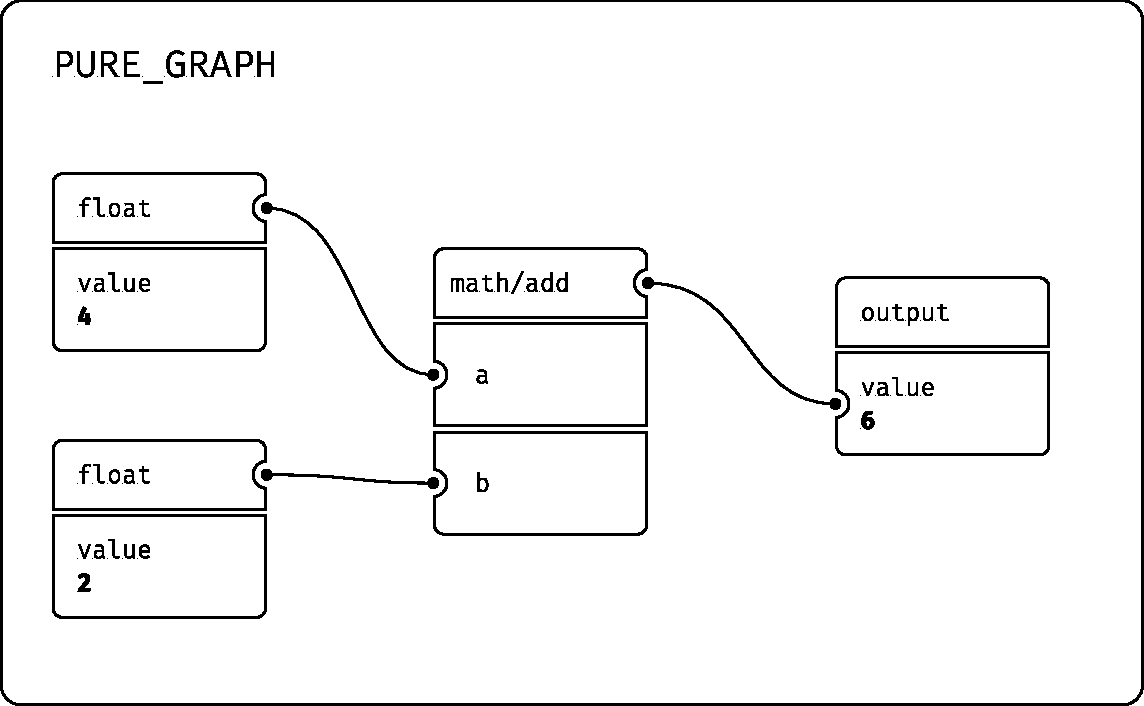
\includegraphics[width=\textwidth]{graphics/PURE_GRAPH.pdf}
        \caption{Darstellung eines \link[node_graph]{Node-Graph}}
        \label{sec:PURE_GRAPH}
    \end{minipage}
\end{figure}

\pagebreak

\subsection{Anforderungen}

Wie in der \hyperref[sec:Zielsetzung]{Zielsetzung} beschrieben, gibt es drei Hauptanforderungen an diese VPL; \textbf{Erweiterbarkeit}, \textbf{Performance} und \textbf{gute User-Experience}.

\subsubsection{Erweiterbarkeit}

Hiermit ist gemeint, dass das System einfach um neue \link[node_definition]{Node-Definitionen} erweitert werden kann.
\qt{Einfach} heißt in diesem Kontext das ein/e andere/r Programmierer/in möglichst 
schnell in der Lage sein soll eigene WebAssembly-Module zu schreiben welche dann von der VPL geladen und ausgeführt werden können.
Um dies zu erreichen müssen die Interfaces und Abstraktionen möglichst minimal gehalten werden.
\br
Außerdem sollen die Komponenten, auf die ich in der \link{Architektur} noch genauer eingehen werde, in unterschiedlichen Umgebungen implementiert und ausgeführt werden können.
Vorstellbar wäre zum Beispiel das der/die Nutzer/in den \link[node_graph]{Node-Graph} in einer Web-App bearbeitet, dieser aber in Echtzeit auf einem Server ausgeführt wird.

Dies erfordert eine möglichst lose Kopplung und die Minimierung des Datentransfers zwischen den einzelnen Komponenten.

\subsubsection{Performance}

Geschwindigkeit von User-Interfaces ist ein wichtiger Indikator für die User-Experience \cite{6876022}. 
Je schneller Nutzende nach einer Änderung das Ergebnis sehen, desto schneller und effizienter können diese iterieren. 

Da diese VPL als Webanwendung entwickelt wird, spielt auch die Ladezeit eine Rolle. 
Hierbei muss darauf geachtet werden diese so kurz wie möglich zu halten.

\subsubsection{User-Experience}

Diese Anforderung ist deutlich schwieriger zu konkretisieren. User-Experience umfasst die gesamte Interaktion von der ersten Interaktion bis zur regelmäßigen Nutzung.
Hierbei spielen Performance, Konsistenz, Fehlermanagement und Feedback eine große Rolle.
\br
\cmt{Hier muss definitiv noch mehr rein}

\subsubsection{Nicht-Ziele}

Die Webplattform als solche bietet viele Möglichkeiten Anwendungen für Nutzer/innen mit Behinderungen angenehmer zu gestalten. 
Die dynamische Struktur einer VPL, sowie spezifische Details der Implementierung machen dies für diese Anwendung ein sehr großes Unterfangen. 
Soweit möglich sollte auf Zugänglichkeit geachtet werden, diese aber umfassend zu garantieren wird nicht Teil dieser Arbeit sein.
\br
Auch die Optimierung für mobile Endgeräte ist nicht vorgesehen, da die Art der Anwendung sich nicht für kleine Bildschirme oder Touch-Interfaces eignet.
\br
Hierbei ist aber zu erwähnen das diese Ziele nur im Kontext der Bachelorarbeit ausgeklammert werden, für zukünftige Weiterentwicklung aber durchaus infrage kommen.

\pagebreak

\subsection{Architektur}
\label{sec:Architektur}

Die Architektur besteht aus drei Hauptkomponenten. 
Das \link[node_interface]{Node-Interface} ist für das visuelle Interface zuständig, hier interagieren Nutzer/innen mit dem \link[node_graph]{Node-Graph}.
\br
Der \link[runtime_executor]{Runtime-Executor} ist für die Ausführung der Nodes zuständig. Er nimmt einen serialisierten \link[node_graph]{Node-Graph} entgegen und gibt das Ergebnis zurück.
\br
Die \link[node_registry]{Node-Registry} ist für das Verwalten der \link[node_definition]{Node-Definitionen} zuständig. Die beiden anderen Komponenten laden aus ihr die einzelnen WebAssembly-Binärdateien der Nodes.
\br
In Abbildung \ref{fig:overview_sequence} ist in einem Sequenzdiagramm dargestellt wie die drei Komponenten zusammenarbeiten.

\begin{figure}[hbtp]
    \centering
    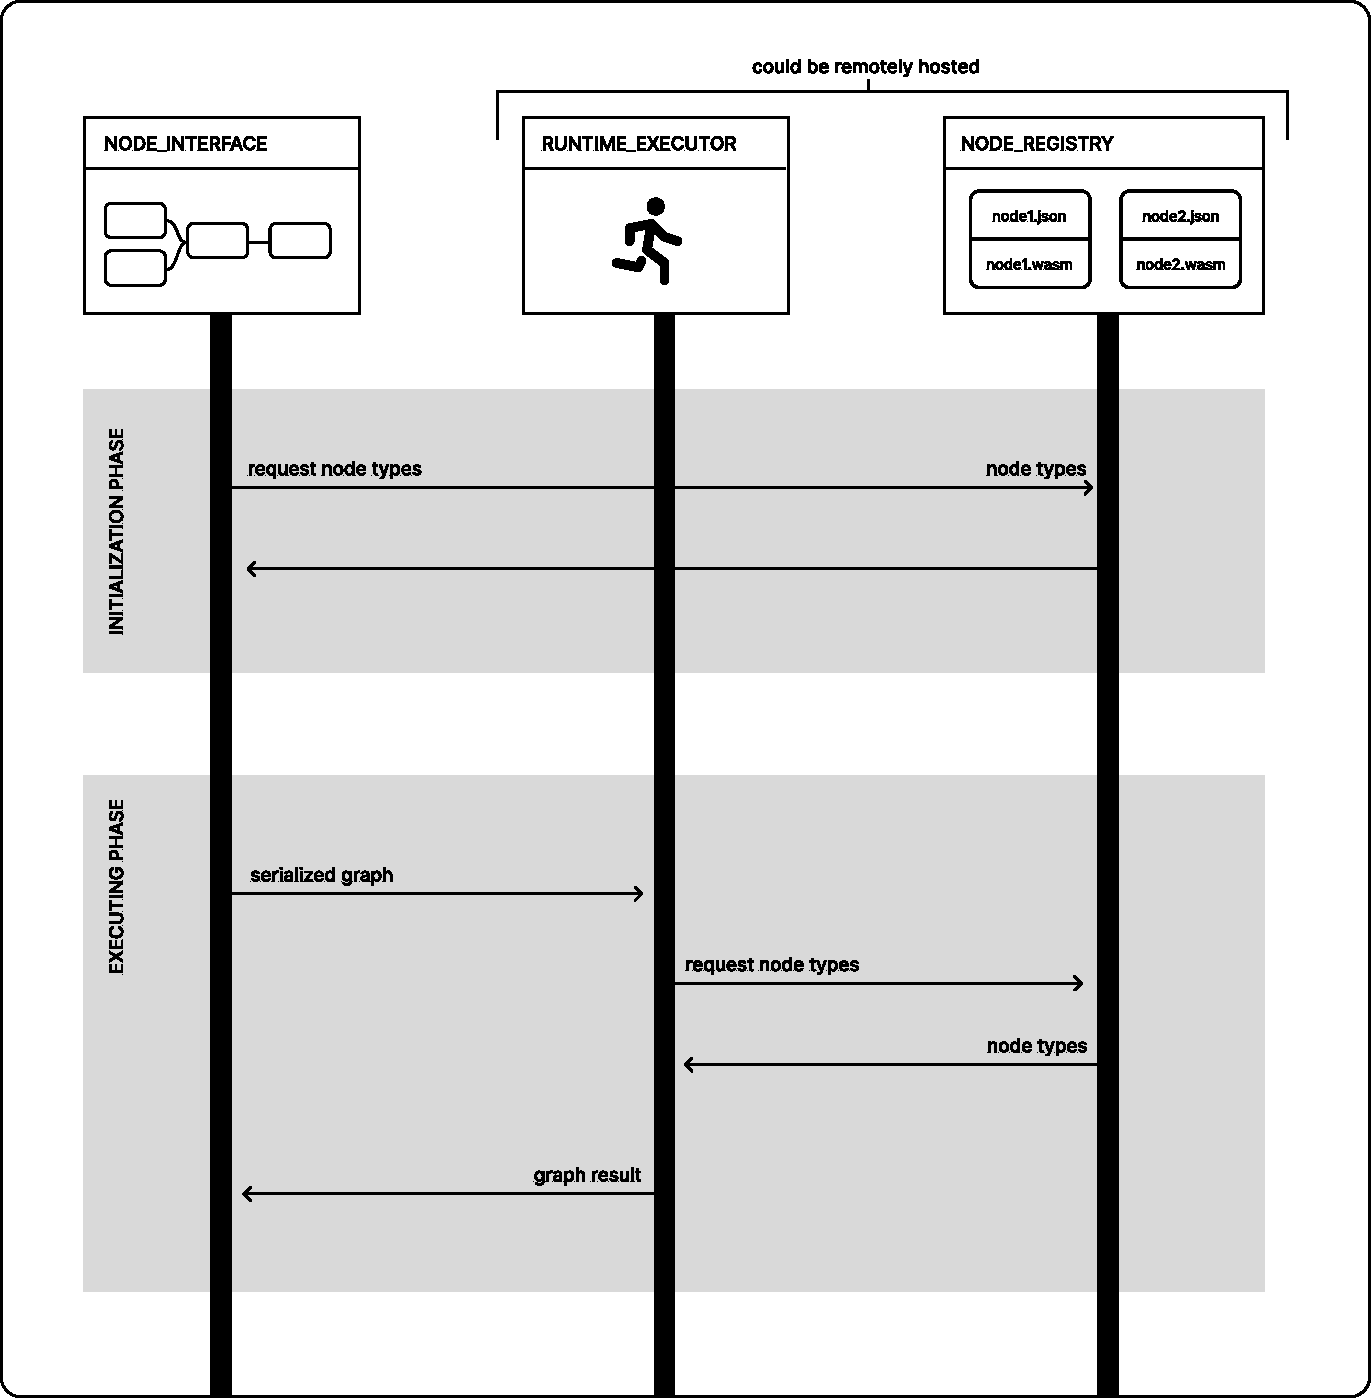
\includegraphics[width=1\textwidth]{graphics/OVERVIEW_SEQUENCE.pdf}
    \caption{Sequenzdiagramm der Architektur}
    \label{fig:overview_sequence}
\end{figure}

\pagebreak

\subsubsection{Datentypen}

Die Datentypen wurden möglichst minimal gehalten. Dies dient zum einen dem Ziel das gesamte System so einfach und verständlich wie möglich zu halten, und zum
anderen macht es die Serialisierung und Deserialisierung der Daten schneller.
\br
Die drei Hauptdatentypen sind  \link[data_node_type]{Node-Definition}, \hyperref[fig:data_node]{Node},  und \hyperref[fig:data_node_graph]{Node-Graph}. 

\subsubsection*{Node-Definition}

\begin{figure}[htbp]
  \begin{code}
    \begin{minted}{typescript}
type NodeDefinition = {
  id: string;
  inputs?: Record<string, NodeInput>
  outputs?: string[];
  execute?: (args: Int32Array) => Int32Array;
}

const mathNodeType: NodeDefinition = {
  id: "max/plantarium/math",
  inputs: { 
    op_type: { type:"select", options: ["add","subtract","multiply","divide"] }, 
    a: { type: "float" }, 
    b: { type: "float" } 
  },
  outputs: ["float"],
  execute: (inputs) => {
    // Implementierung der Math Node
  }
}
    \end{minted}
  \end{code}

  \caption{Datenstruktur der \link[node_definition]{Node-Definition} (TypeScript)}
  \label{sec:data_node_type}

\end{figure}

Die Node-Definition besteht aus einer \topic{id}, \topic{inputs}, \topic{outputs} und einer \topic{execute} Funktion. Die \topic{inputs} einer \link[node]{Node} können unterschiedliche \topic{type} Werte haben:

\begin{itemize}
  \setlength\itemsep{0.0em}
  \item float
  \item integer
  \item boolean
  \item select
  \item vec3
  \item etc.
\end{itemize}

Über diese \topic{inputs} legen die Nutzer fest welche Argumente eine \link[node]{Node} entgegennimmt.
Im \link[node_interface]{Node-Interface} werden diese dann als Eingabefelder dargestellt. Außerdem legen diese Inputs fest welche \link[node]{Nodes} mit dieser \link[node]{Node} verbunden werden können. 
\br
Ein weiteres Attribut eines \topic{inputs} ist \topic{setting}. So können die Nutzer Argumente festlegen die global für den ganzen \link[node_graph]{Node-Graph} gelten und nicht direkt von einer \link[node]{Node} abhängen. Ein Beispiel aus der Entwicklung wäre hier die \topic{resolution}. Diese legt fest wie viele Vertices eine \link[node]{Node} für ein 3D-Modell generieren soll. Das \link[node_interface]{Node-Interface} konstruiert aus allen \topic{settings} ein globales Einstellungsmenü.
\br
Außerdem gibt es bestimmte Input-Typen die besondere Funktionen haben. So kann eine \link[node]{Node} zum Beispiel einen Input mit \topic{\{"type":\\"\\seed"\}} festlegen, und diesem wird bei der Ausführung durch den \link[runtime_executor]{Runtime-Executor} ein zufälliger Wert zugewiesen.
\br
Einige andere Attribute wurden ausgeklammert um die Lesbarkeit zu erhöhen. So kann ein \topic{input} noch ein \topic{label}, ein \topic{default} und eine \topic{description} haben.

\subsubsection*{Node}

\begin{figure}[htbp]
  \begin{code}
    \begin{minted}{typescript}
type Node = {
  id: number;                       // Primäre ID der Node
  type: string;                     // Type der Node, bsp: max/plantarium/math
  props?: Record<string, any>,      // Daten der Node
  position: [x: number, y: number]  // Visuelle Position
}

const exampleNode: Node = {
  id: 5,
  type: "max/plantarium/math",
  props: { op_type: 0, a: 400, b: 20},
  position: [60, 90]
}

    \end{minted}
  \end{code}

  \caption{Datenstruktur einer \link[node]{Node} (TypeScript)}
  \label{fig:data_node}

\end{figure}

Eine \link[node]{Node} ist eine Instanz einer \link[node_definition]{Node-Definition}. Die Datenstruktur besteht aus einer \topic{id}, einem \topic{type}, optionalen \topic{props} und einer \topic{position}. 
Dieser Datentype findet vorallem Anwendung im \link[node_interface]{Node-Interface}, während der Laufzeit und der Serialisierung und Deserialisierung.
\br
Die \topic{id} ist inkrementell und dient zur eindeutigen Identifikation der Node. Der \topic{type} verbindet eine \link[node]{Node} mit einer \link[node_definition]{Node-Definition}.
Die \topic{props} sind die Argumente die an die \topic{execute} Funktion der \link[node_definition]{Node-Definition} übergeben werden.

\subsubsection*{Node-Graph}

\begin{figure}[htbp]
  \begin{code}
    \begin{minted}{typescript}
type NodeGraph = {
  id: number;                                 // Primäre ID des Graphen
  nodes: Node[];                              // Liste aller Nodes
  edges: [number, number, string][];  // Liste aller Verbindungen
}
    \end{minted}
  \end{code}

  \caption{Datenstruktur eines \link[node_graph]{Node-Graph} (TypeScript)}
  \label{fig:data_node_graph}

\end{figure}

Der \link[node_graph]{Node-Graph} besteht aus einer \topic{id}, einer Liste aller \link[node]{Nodes} und einer Liste aller Verbindungen. 
Die Verbindungen sind jeweils ein Tupel aus der \topic{id} der \link[node]{Node} von der die Verbindung ausgeht, der \topic{id} der \link[node]{Node} zu der die Verbindung geht, und der \topic{id} des \topic{inputs} der empfangenden Node.

\pagebreak

\subsubsection{Node-Interface}
\label{sec:node_interface}
\cmt{Visuelles Interface für den Node-Graph}
\subsubsection{Node-Registry}
\label{sec:node_registry}
\cmt{Verwaltung der Nodes}
\subsubsection{Runtime-Executor}
\label{sec:runtime_executor}
\cmt{Ausführung der Nodes}

\pagebreak

\subsubsection{Higher Order Nodes / Parameter}
\label{sec:HON}
In vorherigen Abschnitten wurde der Vergleich zwischen \link[node]{Nodes} und Funktionen gezogen. Dies hat den Vorteil, dass es das Konzept etwas leichter verständlich macht.
Es gibt jedoch Situationen, in denen es sinnvoll ist, von dem Konzept einer Node als reiner Funktion abzuweichen, damit die VPL zum einen flexibler und zum anderen einfacher zu bedienen ist.
\subsubsection*{Random Problem}
Wie in Abbildung \ref{fig:random_problem} dargestellt, würde das Ergebnis der \topic{random} Node identisch sein, wenn sie nur einmal ausgeführt wird, unabhängig davon, wie viele \topic{math/add} Nodes als Empfänger dienen. 
Eine mögliche Lösung wäre, die \topic{random} Node für jede ihrer ausgehenden Verbindungen separat auszuführen. 
Dies könnte jedoch zur unnötigen Mehrfachausführung von Nodes führen, die dies nicht erfordern.
Außerdem erschwert dies das Caching von Node-Ergebnissen, da nicht nur die Node-Parameter, sondern auch die Anzahl der Verbindungen das Ergebnis beeinflussen würden.
\br
Ein weiterer Nachteil ist das für dieses Konzept die Ausführung der Nodes nicht mehr nur in eine Richtung verläuft. Das könnte zu konzeptioneller Verwirrung und Komplexität führen.
\br
\begin{figure}[htbp]
  \centering
  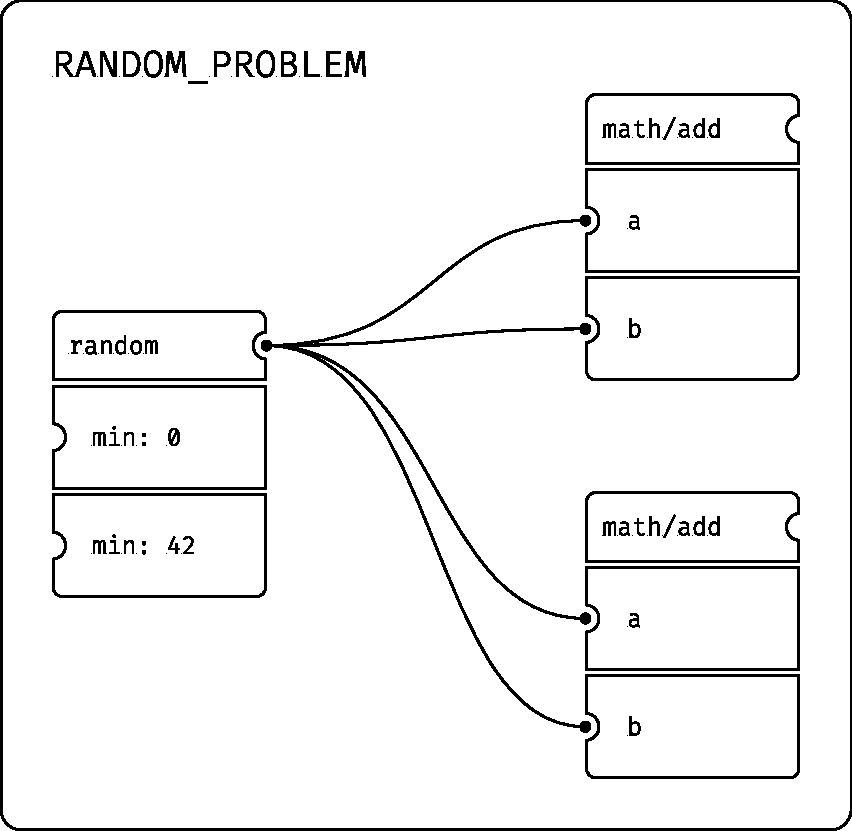
\includegraphics[width=0.5\textwidth]{graphics/RANDOM_PROBLEM.pdf}
  \caption{Illustration eines Problems mit der \texttt{random} Node}
  \label{fig:random_problem}
\end{figure}

\pagebreak

\subsubsection*{Noise Problem}

Ein weiteres Problem soll durch Abbildung \ref{fig:noise_problem} verdeutlicht werden. 
Die hypothetische \topic{cylinder} Node generiert 3D-Modelle von Zylindern. Sie hat einen Input für den Radius, die Höhe und die Anzahl der generierten Zylinder. 
\br
Wenn die vorherigen Nodes als pure Funktionen modelliert wären, gäbe es für sie jeweils nur ein Ergebnis und die \topic{cylinder} Node würde 10 identische Zylinder generieren.

\begin{figure}[htbp]
  \centering
  \includegraphics[width=0.8\textwidth]{./graphics/NOISE_PROBLEM.pdf}
  \caption{Problemdarstellung}
  \label{fig:noise_problem}
\end{figure}

\subsubsection*{Lösung}

Eine Lösung für dieses Problem ist die Einführung von parametrisierten Nodes. Das heißt bestimmte Nodes geben kein Ergebnis zurück, sondern eine parametrisierte Version ihrer selbst, die dann von anderen Nodes evaluiert werden kann.
\br
Dies hat den entscheidenden Vorteil das andere Nodes frei entscheiden können, wo und wie oft sie ihre Argumente evaluieren.
Des Weiteren können diese Nodes wiederum eigene Argumente bei der Evaluierung übergeben.
\br
Die \topic{cylinder} Node im vorherigen Beispiel könnte zum Beispiel bei der Evaluierung der \topic{random} Node ein \topic{seed} übergeben.
\br
Eine Herausforderung in der Implementierung dieser Lösung besteht darin das jedes Argument nun entweder ein direkter Wert, der von den Nutzern über das \link[node_interface]{Node-Interface} festgelegt wird, oder ein Teil das gesamten \link[node_graph]{Node-Graphen} sein kann.
\br
Da der \link[runtime_executor]{Runtime-Executor} aus Gründen der Erweiterbarkeit möglichst wenig spezifische Informationen über einzelne Nodes brauchen soll,
habe ich mich dazu entschieden das die einzelnen Nodes sich selber serialisieren und diese Serialisierung als Ergebnis zurückgeben.
\br
Die erste Implementierung bestand darin das die Nodes ein serialisiertes JSON-Objekt zurückgeben. Dies hatte den Vorteil, dass einzelne Argumente zu Debugging-Zwecken menschenlesbar und die Serialisierung relativ einfach war. Die Performance war jedoch nicht optimal, da die Serialisierung und Deserialisierung relativ aufwendig ist. Des Weiteren hatte jede Node jetzt eine Abhängigkeit zu \href{ https://serde.rs/ }{Serde} (Der Standardbibliothek für Serialisierung in Rust), was die Dateigröße der WebAssembly-Module deutlich vergrößerte.
\br
Die aktuelle Version benutzt eine eigene Binär-Serialisierung. Diese ist schneller und die Dateigröße der WebAssembly-Module ist kleiner. Der Nachteil ist das die Serialisierung nicht mehr menschenlesbar und die Implementierung komplexer ist. 
\\
Die Grundidee ist es Nodes als ein Array aus 32Bit Integer darzustellen, die erste Stelle des Arrays enkodiert den Typ der Node, die darauffolgenden Stellen sind die Argumente. Die einzelnen Argumente sind entweder eine Zahl oder die enkodierte Version einer anderen Node.
Gleitzahlen sind 32 Bit nach dem IEEE-754 Standard und können dank der gleichen Größe ohne weiter Anpassungen im Array gespeichert werden. 
\br
Da WebAssembly, sowie auch Rust keine verschachtelten Arrays unterstützen, muss dieser Array in einen linearen Array umgewandelt werden. 
Der \qt{Recursive-Length Prefix Serialization} Algorithmus von Ethereum war ein guter Ansatz, jedoch nicht für die Anforderungen dieser Anwendung optimiert, da er für Strings ausgelegt ist. 
\cite{wood2024ethereum}
\br
Das aktuelle Binärformat besteht darin jede Klammer in einer verschachtelten Struktur durch zwei 32 Bit Integer zu enkodieren. 
Die erste Stelle gibt, an ob es sich um eine öffnende oder schließende Klammer handelt, die zweite Stelle gibt den Abstand zur nächsten Klammer an.

\begin{figure}[htbp]
  \begin{code}
    \begin{minted}{typescript}
const input = [ 0, 2, 3, [ 2, [ 5 ] ] ]

const endoded = [
  0, // 0 => Klammer auf
  3, // Abstand zur nächsten Klammer
  2,
  3,
  0, // 0 => Klammer auf
  2, // Abstand zur nächsten Klammer
  2, 
  0, // 0 => Klammer auf
  2, // Abstand zur nächsten Klammer
  5,
  1, // 1 => Klammer zu
  1, // 1 => Klammer zu
  1, // 1 => Klammer zu
  1, // 1 => Klammer zu
  1, // 1 => Klammer zu
  1, // 1 => Klammer zu
]

    \end{minted}
  \end{code}

  \caption{Beispiel einer Binär-Serialisierung}
  \label{sec:data_nested_encoding}

\end{figure}

Eine Limitierung dieser Implementierung ist das 32 Bit integer nur Zahlen bis maximal $2^{31}-1$ darstellen können. Dies beschränkt die Länge eines Arrays auf $2,147,483,647$ Elemente. Für diese Anwendung ist dies jedoch mehr als ausreichend.

\subsubsection*{O-Notation}
Die O-Notation der \link[code_nested_encoding]{Beispiel-Implementierung} ist $O(n)$, wobei $n$ die Anzahl der Elemente in der Serialisierung ist. Während der Serialisierung der einzelnen \link[node]{Nodes} muss aber nicht der gesamte Array deserialisiert und serialisiert werden. Hier können wir den serialiserten Input in einzelne Argumente \link[code_nested_splitting]{aufteilen} und diese am Ende wieder \link[code_nested_joining]{zusammenfügen}. Dies hat den Vorteil das die Serialisierung und Deserialisierung von einzelnen Argumenten $O(1)$ ist.

\subsection{Technologien}
\subsubsection{WASM-Bindgen}
\label{sec:WASM-Bindgen}
\subsubsection{Svelte}
\label{sec:Svelte}
\subsubsection{Rust}
\label{sec:Rust}
\subsubsection{TypeScript}
\label{sec:TypeScript}
\subsubsection{WebAssembly}
WebAssembly (WASM) ist ein Bytecode-Format für eine Stack-basierte virtuelle Maschine. Es wurde von der WebAssembly Working Group des World Wide Web Consortium (W3C) entwickelt und ist seit 2017 ein offizieller Web-Standard \cite{Haas2017}. 
\br
Es wird hauptsächlich als Kompilierungsziel für kompilierte Programmiersprachen wie C, C++ und \link[Rust]{Rust} benutzt, um diese in Webanwendungen zu integrieren. Im Gegensatz zu Javascript ist WebAssembly nicht garbage-collected und ist außerdem stark typisiert. Dies ermöglicht es, performante und sicherere Anwendungen zu entwickeln.
\linebreak
\textbf{WASI}
\cmt{WebAssembly System Interface}
\linebreak
\textbf{WAT}
\cmt{WebAssembly Text Format}
\linebreak
\textbf{WebAssembly Component Model}
\cmt{Kind of like ES-Modules or C-Style Linking}
\linebreak
\textbf{WIT}
\cmt{WebAssembly Interface Types}

\subsection{Design}

\section{Implementierung}
\subsection{UI}
\subsection{Backend}

\section{Evaluation}
\section{Fazit}

\pagebreak
\section{Glossar}

\subsection{Node}
\label{sec:node}
Einzelner Baustein eines \hyperref[sec:node_graph]{Node-Graphs}. Eine Node funktioniert etwa wie eine Funktion in einer textuellen Programmiersprache. Sie nimmt \hyperref[sec:node_argumente]{Node-Argumente} entgegen, verarbeitet diese und gibt ein Ergebnis zurück. 

\begin{figure}[htbp]
    \centering
    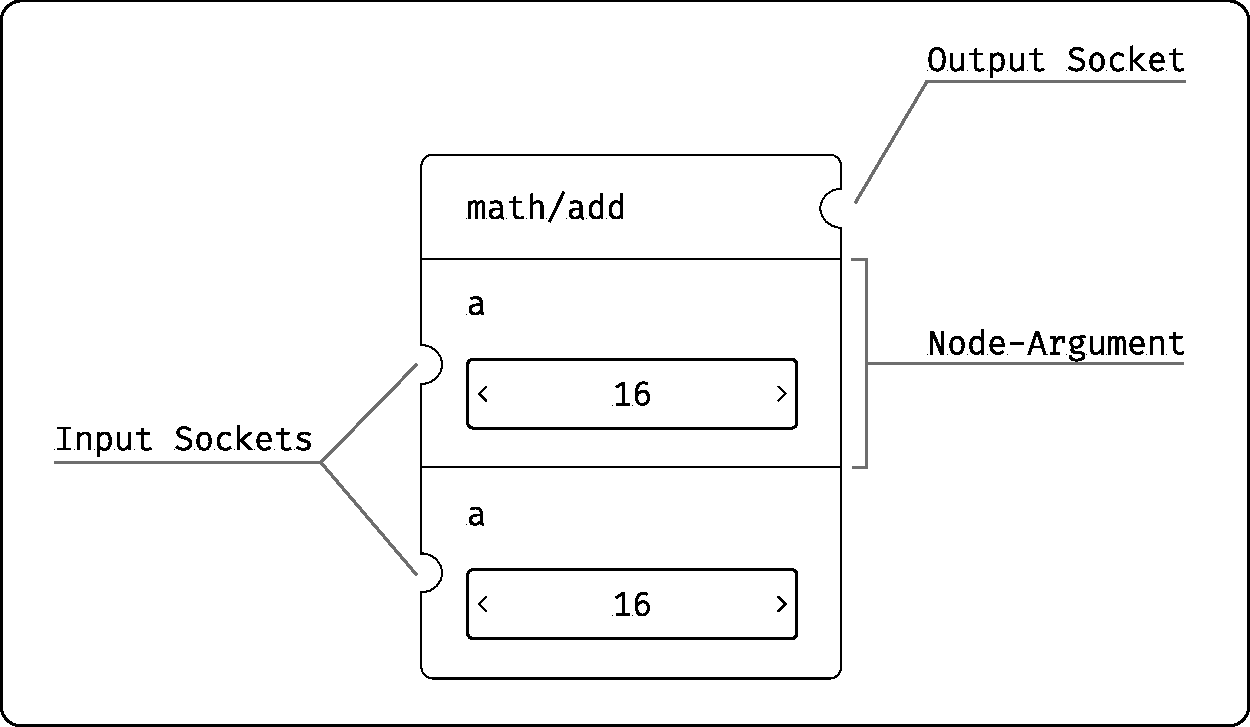
\includegraphics[width=0.8\textwidth]{graphics/NODE_ANATOMY.pdf}
    \caption{Anatomie einer Node}
    \label{sec:NODE_ANATOMY}
\end{figure}

\subsection{Node-Definition}
\label{sec:node_definition}
Eine Node ist quasi eine Instanz einer Node-Definition. Eine Node-Definition definiert die Struktur einer Node. Sie enthält Informationen über die Inputs und Outputs einer Node und die Funktion, die die Node ausführt.

\subsection{Node-Graph}
\label{sec:node_graph}
Node-Graphs sind ein gerichteter \link[PURE_GRAPH]{azyklischer Graph (DAG)} von \link[node]{Nodes}. Sie bestehen aus einer Menge von Nodes und deren Verknüpfungen. 

\subsection{Node-Argumente}
\label{sec:node_argumente}
Node-Argumente sind die Eingabeparameter einer Node. Ein Node-Argument kann entweder direkt über das Interface in einer \link[node]{Node} definiert werden oder indem der User einen Output-Socket einer anderen Node mit dem \link[node_socket]{Node-Socket} eines Node-Argument verknüpft.

\subsection{Node-Socket}
\label{sec:node_socket}
Node-Sockets sind die Verbindungspunkte zwischen \link[node]{Nodes}. Eine Node hat mehrere Input-Sockets und einen Output Socket.

\section{Beispiel-Code}

\subsection{Binär-Serialisierung}
\label{sec:code_nested_encoding}

\begin{figure}[htbp]
  \begin{code}
    \begin{minted}{typescript}
// Recursiver Datenstruktur für verschachtelte Arrays
type SparseArray = (number | number[] | SparseArray<T>)[];

// Kodiert ein verschachteltes Array
export function encodeNestedArray(array: SparseArray): number[] {
  const encoded = [0, 0]; // Initialisiere das Ergebnis
  let missingBracketIndex = 1; // Abstand zur letzten Klammer

  for (let index = 0; index < array.length; index++) {
    const item = array[index];
    if (Array.isArray(item)) {
      // Aktualisiere die letzte Klammer
      encoded[missingBracketIndex] = encoded.length - missingBracketIndex;
      if (item.length === 0) {
        // Behandle leere Arrays
        encoded.push(0, 1, 1, 1);
      } else {
        // Kodiere rekursiv nicht-leere Arrays
        const child = encodeNestedArray(item);
        encoded.push(...child);
      }
      // Aktualisiere den Abstand für die zuletzt geöffnete Klammer
      missingBracketIndex = encoded.length - 1;
    } else {
      // Behandle Nicht-Array-Elemente
      encoded.push(item);
      // Aktualisiere den Abstand für die zuletzt geöffnete Klammer
      if (missingBracketIndex) encoded[missingBracketIndex] = index + 2;
    }
  }

  return [...encoded, 1, 1];
};
    \end{minted}
  \end{code}

  \caption{Beispiel-Code Binär-Serialisierung}
  \label{sec:data_nested_encoding}

\end{figure}

\pagebreak

\subsection{Binär-Splitting}
\label{sec:code_nested_splitting}

\begin{figure}[htbp]
  \begin{code}
    \begin{minted}{rust}
pub fn split_args(args: &[i32]) -> Vec<&[i32]> {
    let mut out_args: Vec<&[i32]> = Vec::new();
    let mut depth = 0;
    let mut i = 0;
    let mut start_index = 0;
    let mut next_bracket_index = 0;
    let len = args.len();

    while i < len {
        // check if we are at a bracket
        if i == next_bracket_index {
            next_bracket_index = i + args[i + 1] as usize + 1;
            // check if the bracket is opening
            if args[i] == 0 {
                if depth == 1 {
                    start_index = i;
                }
                depth += 1;
            } else {
                depth -= 1;
                if depth == 1 {
                    out_args.push(&args[start_index..i + 2]);
                    start_index = i + 2;
                }
            }
            i += 2;
            continue;
        } else if depth == 1 {
            out_args.push(&args[i..i + 1]);
            start_index = i + 1;
        }
        i += 1;
    }

    out_args
}
    \end{minted}
  \end{code}

  \caption{Beispiel-Code Binär-Splitting}

\end{figure}

\pagebreak

\subsection{Binär-Joining}
\label{sec:code_nested_joining}
\begin{figure}[htbp]
  \begin{code}
    \begin{minted}{rust}
pub fn concat_args(data: Vec<&[i32]>) -> Vec<i32> {
    // Start with 4 to account for opening/closing brackets
    let mut total_length = 4; 

    for vec in &data { // Calculate the total length first to avoid reallocations
        if vec.len() == 1 {
            total_length += 1;
        } else {
            total_length += vec.len(); // +4 for [0, 1] and [1, 1] per inner vec
        }
    }

    let mut result = Vec::with_capacity(total_length);

    result.push(0); // Add [0, 1] initially
    result.push(1);

    let mut last_closing_bracket = 1;

    for vec in data.iter() { // Process each vector
        if vec.len() == 1 {
            result.push(vec[0]);
            result[last_closing_bracket] += 1;
            continue;
        } else {
            result.extend_from_slice(vec);
            last_closing_bracket = result.len() - 1;
            result[last_closing_bracket] = 1;
        }
    }

    result.push(1); // Add [1, 1] at the end
    result.push(1);

    result
}

    \end{minted}
  \end{code}

  \caption{Beispiel-Code Binär-Joining}

\end{figure}

\pagebreak
\section{Literaturverzeichnis}

\printbibliography

\end{document}
